\chapter{Análise empírica}\label{cap:analise-empirica}
Este capítulo tem como objetivo analisar empiricamente todos os algoritmos de ordenação apesentados anteriormente, comparando a análise teórica com os resultados obtidos na prática, no que diz respeito ao tempo de execução, número de comparações e número de movimentações.

\section{Preliminares}
Nesta seção, descreve-se o ambiente de desenvolvimento, indicando o hardware e os softwares utilizados na implementação dos algoritmos e na execução dos testes. Também é apresentada a organização do projeto em diretórios e arquivos. Além disso, são feitas definições necessárias para o melhor entendimento das seções seguintes. Por fim, descreve-se o que foi coletado e como essa coleta foi realizada.

\subsection{Ambiente de desenvolvimento}
Para a implementação dos algoritmos e execução dos testes foi utilizado o notebook descrito na Tabela \ref{tab:hardware-and-softwares}. Todos os algoritmos e funções auxiliares foram implementados com a linguagem de programação C. As linguagens de programação Bash e Python foram utilizadas de forma secundária para automatização dos testes e geração de gráficos, respectivamente. O hardware, softwares e versões utilizados são especificados na tabela \ref{tab:hardware-and-softwares}.

\begin{table}[H]
    \centering
    \Caption{\label{tab:hardware-and-softwares}Hardware e softwares utilizados}
    \begin{tabular}{ | c | l | l | }
        \hline
        Tipo                      & Componente                & Produto                          \\
        \hline
        \multirow{3}{*}{Hardware} & Modelo                    & Avell A65i                       \\
                                  & Processador               & 13th Gen Intel® Core™ i9-13900HX \\
                                  & Cache                     & 36 MB Intel® Smart Cache         \\
                                  & Memória principal         & 64.0 GiB                         \\
        \hline
        \multirow{4}{*}{Software} & Sistema operacional       & Linux Ubuntu 24.04.3 LTS         \\
                                  & Editor de texto           & Microsoft Visual Studio Code     \\
                                  & Compilador C              & GNU Compiler Collection GCC      \\
                                  & Linguagens de programação & C, Bash e Python                 \\
        \hline
    \end{tabular}
\end{table}

\subsection{Organização do código fonte}
A figura \ref{fig:projeto-ordenacao} ilustra a forma como código fonte do projeto foi organizado, enquanto que a tabela \ref{tab:projeto-ordenacao} dá uma breve descrição de cada arquivo.

\begin{figure}[H]
\Caption{\label{fig:projeto-ordenacao}Árvore de diretórios e arquivos do projeto}
\centering
\begin{forest}
    for tree={font=\ttfamily, grow'=0,
    folder indent=.9em, folder icons,
    edge=densely dotted}
    [
        [graficos
            [graficos.ipynb, is file]
        ]
        [scripts
            [testes.sh, is file]
        ]
        [src
            [main.c, is file]
            [ordenacao.c, is file]
            [ordenacao.h, is file]
        ]
        [.gitignore, is file]
        [README.md, is file]
    ]
\end{forest}
\vspace{3pt}
\Fonte{Elaborado pelo autor. Acesso público em https://github.com/jbrenorv/ordenacao}
\end{figure}

\begin{table}[H]
    \centering
    \Caption{\label{tab:projeto-ordenacao}Descrição dos arquivos do projeto}
    \begin{tabular}{ | c | l | }
        \hline
        Arquivo        & Descrição                                                       \\
        \hline
        graficos.ipynb & Arquivo exportado do notebook criado no Google Colab            \\
        testes.sh      & Implementa script em Bash para execução automatizada dos testes \\
        main.c         & Implementa a função principal                                   \\
        ordenacao.c    & Implementa os algoritmos de ordenação e funções utilitárias     \\
        ordenacao.h    & Declara os protótipos dos algoritmos e funções utilitárias      \\
        .gitignore     & Declara diretórios e arquivos que o Git deve ignorar            \\
        README.md      & Documenta o projeto com instruções de execução dos testes       \\
        \hline
    \end{tabular}
\end{table}

\subsection{Tipos de vetores}
Além do tamanho do vetor, a forma como os elementos estão dispostos inicialmente pode interferir no tempo e na quantidade de operações que cada algoritmo executa. Pensando nisso, com o objetivo de analisar como cada algoritmo se comporta para diferentes tipos de entrada, foram considerados três tipos de vetores nos testes, como mostra a tabela \ref{tab:tipos-de-vetores}.

\begin{table}[H]
    \centering
    \Caption{\label{tab:tipos-de-vetores}Tipos de vetores}
    \begin{tabular}{ | c | l | }
        \hline
        Tipo   & Descrição                                \\
        \hline
        1      & Vetores já ordenados em ordem crescente  \\
        2      & Vetores ordenados em ordem decrescente   \\
        3      & Vetores gerados de forma pseudoaleatória \\
        \hline
    \end{tabular}
\end{table}

\subsection{Dados coletados}
Esta seção visa apenas apresentar e definir quais dados foram coletados. A próxima seção descreve com mais detalhes como a coleta foi realizada. Para cada combinação de algoritmo, tamanho e tipo de vetor, foi registrado o número de comparações, o número de movimentações e o tempo de execução. Essas três métricas são definidas na tabela \ref{tab:dados-coletados}.

Obter essas informações de cada algoritmo é importante para sabermos na prática como eles se comportam para diferentes configurações de entrada. Por exemplo, um algoritmo que executa muitas movimentações pode não ser adequado em um cenário em que mudar os registros de posição seja uma operação muito lenta.

\begin{table}[H]
    \centering
    \Caption{\label{tab:dados-coletados}Dados coletados e suas definições}
    \begin{tabular}{ | c | l | }
        \hline
        Dado                    & Definição                                                     \\
        \hline
        Número de comparações   & \makecell[l]{Uma comparação ocorre quando um elemento do      \\
                                               vetor é comparado com outro elemento do vetor ou \\
                                               com outra variável do programa}                  \\
        Número de movimentações & \makecell[l]{Uma movimentação ocorre sempre que um valor é    \\
                                               atribuído a um elemento do vetor ou um elemento  \\
                                               do vetor é atribuído a uma outra variável}       \\
        Tempo de execução       & \makecell[l]{Tempo decorrido entre o início e o fim da        \\
                                               execução do algoritmo em segundos}               \\
        \hline
    \end{tabular}
\end{table}

\subsection{Metodologia de coleta}
\subsubsection{Entrada}
A função principal é o ponto de entrada para qualquer programa escrito em linguagem de C. De uma forma mais técnica, ao compilar e linkar o código fonte do projeto, obtém-se um arquivo binário executável que, ao ser executado, invoca a função principal para iniciar a execução do processo. Essa função recebe dois argumentos quando invocada. O primeiro é um número inteiro comumente chamado de argc, que indica a quantidade de parâmetros recebidos. Já o segundo é uma lista de vetores de caracteres comumente chamado de argv, que são os parâmetros em si. O primeiro parâmetro é sempre o nome do arquivo executável ou o caminho absoluto até ele. A tabela \ref{tab:main-parametros} indica os parâmetros adicionais esperados.
\begin{table}[H]
    \centering
    \Caption{\label{tab:main-parametros}Parâmetros da função principal}
    \begin{tabular}{ | c | l | }
        \hline
        Posição (argv) & Parâmetro esperado                                      \\
        \hline
        0              & Nome ou caminho para o arquivo executável               \\
        1              & Nome do arquivo onde deve ser escrito os resultados     \\
        2              & Número representando o tamanho do vetor                 \\
        3              & Número igual a 1, 2 ou 3, representando o tipo do vetor \\
        4              & Número representando número da execução                 \\
        \hline
    \end{tabular}
\end{table}

O último parâmetro, que indica o número da execução, é explicado na subseção \ref{subsection:Testes}, que apresenta como os testes foram executados.

\subsubsection{Processamento}
O processamento consiste na execução sequencial das etapas necessárias para realizar os experimentos definidos neste trabalho. O pseudocódigo apresentado a seguir oferece uma visão de alto nível do fluxo executado pela função principal, desde a leitura dos parâmetros de entrada até o registro dos resultados obtidos. Optou-se por essa forma de apresentação para destacar a lógica geral do procedimento e evitar a exibição detalhada de trechos de código que não contribuem significativamente para a compreensão do funcionamento do sistema.

\begin{algorithm}[H]
    \caption{Função principal}\label{alg-main:cap}
    \DontPrintSemicolon
    \Entrada{A tupla $(S, N, T, E)$ representado os parâmetros listados na tabela \ref{tab:main-parametros}}
    \Inicio{
        $F \gets$ Abre arquivo $S$\;
        $O \gets$ Aloca vetor de tamanho $N$ com valores de acordo com o tipo $T$\;
        $V \gets$ Aloca vetor de tamanho $N$\;
        $L \gets$ Cria lista de pares de algoritmos\footnote{O primeiro elemento é o algoritmo original e o segundo é a versão modificada para obter o número de comparações e movimentações.}\;
        \Para{cada par $(A, A') \in L$}{
            $V \gets$ Cópia de $O$\;
            $t \gets$ Executa $A$ em $V$\footnote{Obtendo o tempo de execução $t$ em segundos.}\;
            $V \gets$ Cópia de $O$\footnote{Neste ponto $V$ está ordenado, então é necessário resetar para o vetor original.}\;
            $(c, m) \gets$ Executa $A'$ em $V$\footnote{Obtendo o número de comparações $c$ e movimentações $m$.}\;
            Adiciona em $F$ uma linha com os resultados\footnote{Precisamente, a linha contêm o nome do algoritmo, o tamanho do vetor, o tipo do vetor, o número da execução, o número de comparações, o número de movimentações e o tempo de execução.}\;
        }
        Libera a memória alocada e fecha o arquivo $F$\;
    }
\end{algorithm}

\subsubsection{Exemplo de saída}
Se após compilar e linkar o código C, o arquivo executável resultante se chamar a.out, o comando a ser executado a partir de um Terminal Linux, aberto no mesmo diretório do executável, poderia ser, por exemplo:
\lstinputlisting[language=bash]{codigos/aux/_bash.txt}
Neste caso, seria gerado um vetor de forma pseudoaleatória (tipo 3) de tamanho 1000 e os resultados seriam escritos no arquivo saida.csv. Com exceção do cabeçalho, o conteúdo do arquivo saida.csv é representado na tabela \ref{tab:exemplo-saida}. Além disso, a coluna do tempo pode conter valores diferentes.
\begin{table}[H]
    \centering
    \Caption{\label{tab:exemplo-saida}Exemplo de saída}
    \begin{tabular}{ | c | l | l | l | l | l | l | }
        \hline
        Algo.        & Tam. & Tipo & Exec. & Comp.  & Movi.  & Tempo (s) \\
        \hline
        Bolha        & 1000 & 2    & 1     & 499497 & 770538 & 0.004037  \\
        Coquetel     & 1000 & 2    & 1     & 388815 & 770538 & 0.003501  \\
        Selecao      & 1000 & 2    & 1     & 499500 & 2958   & 0.000543  \\
        Insercao     & 1000 & 2    & 1     & 257838 & 258844 & 0.000163  \\
        Shellsort    & 1000 & 2    & 1     & 13061  & 20296  & 0.000111  \\
        Mergesort    & 1000 & 2    & 1     & 8717   & 19302  & 0.000098  \\
        Heapsort     & 1000 & 2    & 1     & 8772   & 14040  & 0.000104  \\
        Quicksort    & 1000 & 2    & 1     & 10345  & 20325  & 0.000103  \\
        QuicksortI   & 1000 & 2    & 1     & 12107  & 17646  & 0.000072  \\
        Introsort    & 1000 & 2    & 1     & 14047  & 9620   & 0.000078  \\
        Countingsort & 1000 & 2    & 1     & 0      & 2000   & 0.155960  \\
        Bucketsort   & 1000 & 2    & 1     & 1050   & 4050   & 0.000037  \\
        RadixsortC   & 1000 & 2    & 1     & 0      & 18000  & 0.000022  \\
        RadixsortB   & 1000 & 2    & 1     & 0      & 45000  & 0.000034  \\
        \hline
    \end{tabular}
\end{table}

\subsubsection{Testes}\label{subsection:Testes}
Neste ponto o código implementado em linguagem C está pronto para ser invocado com diferentes parâmetros de entrada. Para automatizar este processo, foi criado um script em linguagem Bash. Este script segue os seguintes passos:
\begin{enumerate}
    \item Compilação do código C e inicialização do arquivo CSV de saída.
    \item Geração dos tamanhos.
    \item Três execuções para cada tamanho e tipo de vetor.
\end{enumerate}

Optou-se por realizar três execuções por tamanho e tipo de vetor para reduzir o impacto de variações ocasionais no tempo de execução, como pequenas flutuações no uso da CPU. Esse número foi escolhido por ser suficiente para obter uma média representativa sem tornar a coleta de dados muito demorada.

Os tamanhos gerados são melhores descritos na tabela \ref{tab:tamanhos}. Foram considerados ao todo $37$ tamanhos entre $10^4$ e $10^8$, inclusive. Além disso, cada tamanho foi usado três vezes para cada um dos três tipos, totalizando $333$ chamadas aos algoritmos.
\begin{table}[H]
    \centering
    \Caption{\label{tab:tamanhos}Geração de tamanhos}
    \begin{tabular}{ | c | l | l | l | c | }
        \hline
        \multicolumn{2}{ | c | }{Intervalo} & \multirow{2}{*}{Incremento} & \multirow{2}{*}{Subtotal} & \multirow{2}{*}{Total} \\
        \cline{1-2}
        Início     & Fim        &        &    &                     \\
        \hline
        $10^4$     & $10^5 - 1$ & $10^4$ & 9  & \multirow{4}{*}{37} \\
        $10^5$     & $10^6 - 1$ & $10^5$ & 9  &                     \\
        $10^6$     & $10^7 - 1$ & $10^6$ & 9  &                     \\
        $10^7$     & $10^8$     & $10^7$ & 10 &                     \\
        \hline
    \end{tabular}
\end{table}

\section{Métodos inferiores}
Os quatro algoritmos classificados neste trabalho como inferiores possuem, como já detalhado em capítulos anteriores, complexidade temporal quadrática no tamanho do vetor de entrada. Eles recebem essa denominação por apresentarem, de acordo com a análise de complexidade apresentada no Capítulo \ref{cap:inferiores}, essa ordem de crescimento. Entretanto, embora todos apresentem a mesma complexidade assintótica, os testes práticos demonstraram que eles possuem desempenhos distintos.

Como o tempo de execução desses algoritmos apresenta crescimento quadrático à medida que o tamanho da entrada aumenta, o tamanho máximo do vetor utilizado foi $n=10^5$. Este tamanho foi considerado razoável para a observação dos resultados esperados, mantendo um tempo de execução viável para os testes.

\subsection{Tempo de execução}
O gráfico a seguir apresenta os resultados de tempo de execução obtidos ao se executar algoritmos de ordenação inferiores.

\begin{figure}[H]
\Caption{\label{fig:inferiores-tempo}Métodos inferiores – Tamanho × Tempo (em segundos).}
\centering
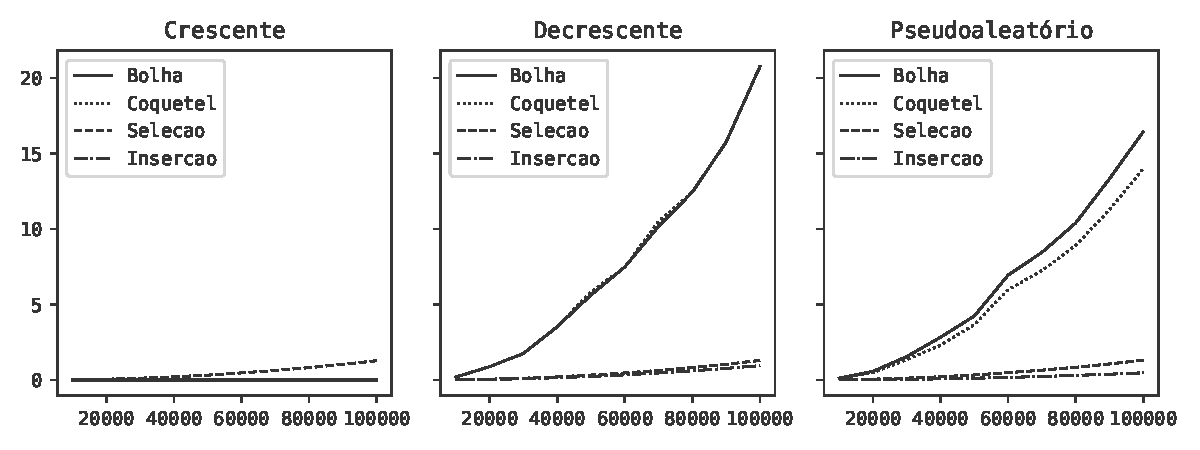
\includegraphics[scale=0.787]{figuras/pdf/inferiores.tempo.pdf}
\Fonte{Elaborado pelo autor}
\end{figure}

Para vetores já ordenados em ordem crescente, como esperado, apenas o algoritmo Selecao chegou a consumir mais de $1s$. Todos os demais algoritmos executaram apenas uma iteração e concluíram suas execuções, o que resultou em um tempo de consumo praticamente nulo.

O pior caso de todos os algoritmos fica evidente para vetores que, inicialmente, estão em ordem decrescente. Curiosamente, no entanto, os algoritmos Bolha e Coquetel se mostraram significativamente mais lentos que o Insercao e o Selecao. O motivo para esse desempenho será detalhado nas próximas seções, onde comparamos o número de comparações e movimentações que cada algoritmo realizou para este tipo de vetor.

Por fim, buscando observar o comportamento geral dos algoritmos, analisamos os vetores gerados de forma pseudoaleatória. Os algoritmos Bolha e Coquetel apresentaram uma leve melhora de desempenho, sendo o Coquetel ligeiramente mais rápido. Isso ocorre porque a iteração de retorno do Coquetel permite que elementos menores atinjam suas posições finais mais rapidamente do que no Bolha. Já os algoritmos Selecao e Insercao foram significativamente mais rápidos, com o Insercao apresentando o melhor resultado geral. Vale notar que o Selecao manteve praticamente o mesmo tempo de execução, independentemente do tipo de vetor. Tal fato se deve à sua característica de sempre executar uma quantidade fixa e quadrática de comparações, enquanto realiza um número mínimo de trocas. Dessa forma, o número de movimentações do Selecao é desprezível no tempo final de execução, o que o torna uma boa escolha para casos em que o vetor possui poucos elementos e a operação de movimentação tem um custo computacional elevado.


\subsection{Comparações}
O gráfico da Figura \ref{fig:inferiores-comparacoes} a seguir, exibe a relação entre o número de comparações e o tamanho do vetor para cada tipo de vetor analisado.

\begin{figure}[H]
\Caption{\label{fig:inferiores-comparacoes}Métodos inferiores – Tamanho × Comparações.}
\centering
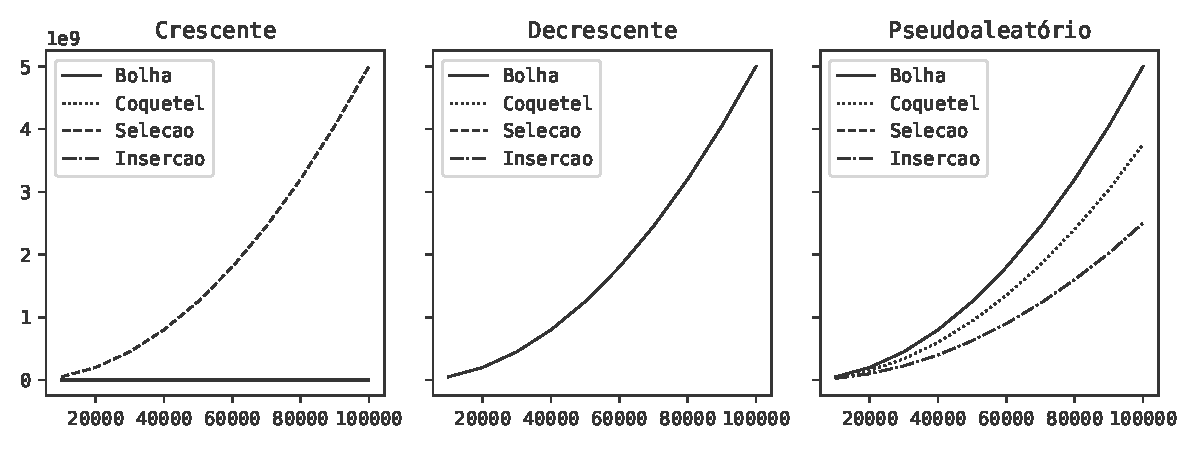
\includegraphics[scale=0.787]{figuras/pdf/inferiores.comparacoes.pdf}
\Fonte{Elaborado pelo autor}
\end{figure}

Para vetores em ordem crescente, como esperado, apenas o algoritmo Selecao executou uma quantidade quadrática de comparações. Os demais algoritmos, por outro lado, executaram uma quantidade linear de comparações, pois levaram apenas uma iteração externa para identificar que o vetor já se encontrava ordenado.

A análise teórica indicava que os algoritmos de ordenação inferiores apresentavam seu pior caso em comum: o vetor ordenado em ordem decrescente. Além disso, ela mostrava que esses algoritmos executam exatamente a mesma quantidade de comparações para esse tipo de vetor. Os testes práticos confirmaram essa conclusão, como é claramente demonstrado no gráfico.

No caso geral, com os vetores gerados de forma pseudoaleatória, pode-se observar que os algoritmos Bolha e Selecao permaneceram praticamente empatados em termos de número de comparações. O algoritmo Insercao demonstrou o melhor resultado, sendo aquele que necessitou do menor número de comparações para finalizar sua execução e garantir um vetor ordenado. Já o Coquetel ficou em um meio-termo, mostrando-se razoavelmente superior ao Bolha e ao Selecao nesse quesito. Sua vantagem reside no fato de que cada iteração externa coloca dois elementos em suas posições finais, além de aproximar os demais elementos de suas posições corretas em pelo menos uma posição.

\subsection{Movimentações}
O gráfico da Figura \ref{fig:inferiores-movimentacoes} a seguir, exibe a relação entre o número de movimentações e o tamanho do vetor para cada tipo de vetor analisado.

\begin{figure}[H]
\Caption{\label{fig:inferiores-movimentacoes}Métodos inferiores – Tamanho × Movimentações.}
\centering
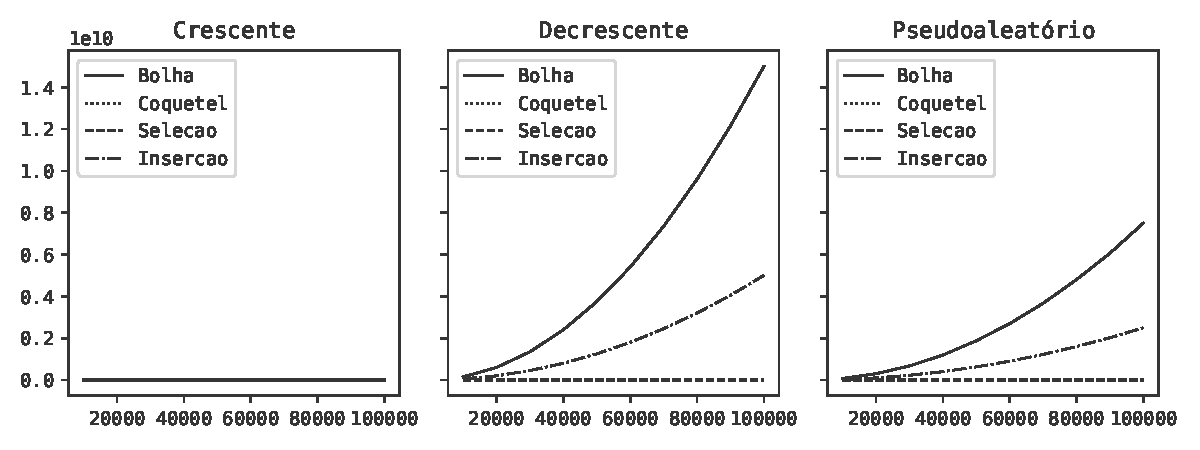
\includegraphics[scale=0.787]{figuras/pdf/inferiores.movimentacoes.pdf}
\Fonte{Elaborado pelo autor}
\end{figure}

Observe que, na prática, independentemente do tipo do vetor, os algoritmos Bolha e Coquetel possuem o mesmo desempenho com relação ao número de movimentações.

Neste ponto, pode-se estabelecer uma boa explicação para o Insercao ter apresentado o menor tempo de execução. Dentre todos os algoritmos inferiores, ele é o que melhor consegue equilibrar o número de comparações e movimentações. Ou seja, ele não possui extremos; enquanto o Bolha e o Coquetel geralmente executam muitas comparações e movimentações, e o Selecao executa muitas comparações e poucas movimentações, o Insercao permanece em um meio-termo. Essa característica o favorece, resultando em um tempo de execução menor que os demais para todos os tipos de vetores.

Quando o assunto é número de movimentações, o Selecao é o algoritmo mais eficiente. Isso ocorre porque ele executa sempre o número mínimo de trocas, garantindo que cada troca posicione pelo menos um elemento em sua posição definitiva. Dessa forma, ele realiza \bigO{n} movimentações, como fica evidente nos gráficos da Figura \ref{fig:selecao-movimentacoes} para todos os tipos de vetores. É importante notar que cada troca executa $3$ movimentações. Observe também que, para vetores decrescentes, cada troca posiciona dois elementos em suas posições finais.

\begin{figure}[H]
\Caption{\label{fig:selecao-movimentacoes}Selecao – Tamanho × Movimentações.}
\centering
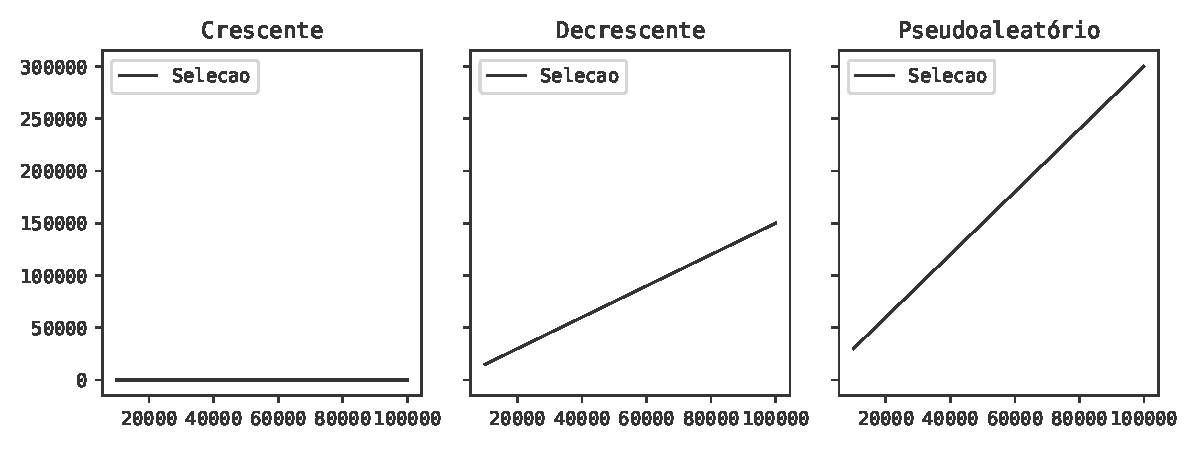
\includegraphics[scale=0.787]{figuras/pdf/selecao.movimentacoes.pdf}
\Fonte{Elaborado pelo autor}
\end{figure}

\section{Métodos superiores}
Os quatro algoritmos classificados como superiores são aqueles que possuem complexidade de tempo de ordem \bigO{n \log n}. Tal complexidade permite a realização de testes com vetores de tamanho consideravelmente maiores do que os utilizados para os algoritmos inferiores, razão pela qual foram testados com vetores cujo tamanho varia de $10^4$ a $10^8$.

\subsection{Tempo de execução}
Foram gerados dois gráficos para apresentar os resultados de tempo de execução. O primeiro, na Figura \ref{fig:superiores1e7-tempo}, mostra os resultados com o tamanho dos vetores limitado a $10^7$, e o segundo, na Figura \ref{fig:superiores1e8-tempo}, apresenta os tamanhos que atingem $10^8$.

\begin{figure}[H]
\Caption{\label{fig:superiores1e7-tempo}Métodos superiores – Tamanho (até $10^7$) × Tempo.}
\centering
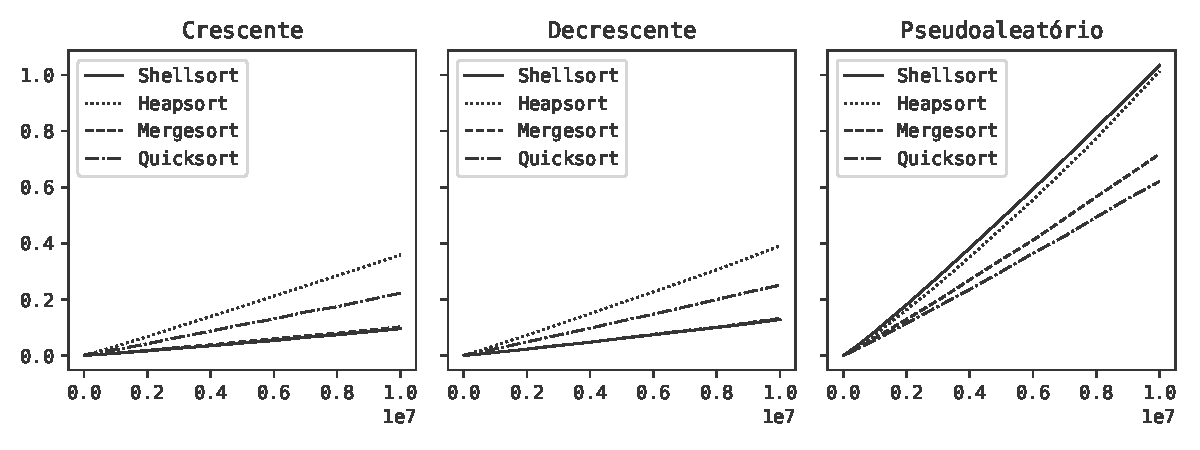
\includegraphics[scale=0.787]{figuras/pdf/superiores1e7.tempo.pdf}
\Fonte{Elaborado pelo autor}
\end{figure}

\begin{figure}[H]
\Caption{\label{fig:superiores1e8-tempo}Métodos superiores – Tamanho (até $10^8$) × Tempo.}
\centering
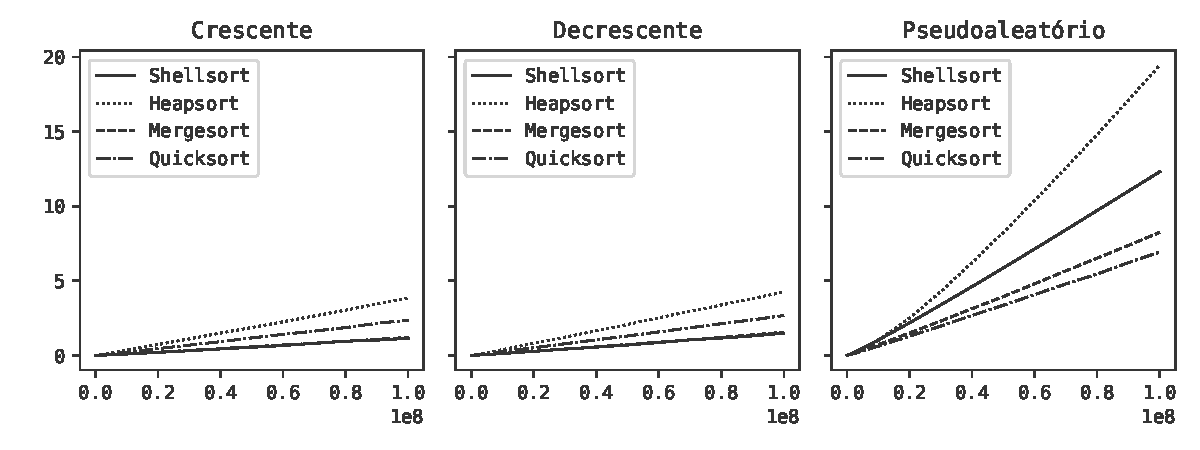
\includegraphics[scale=0.787]{figuras/pdf/superiores1e8.tempo.pdf}
\Fonte{Elaborado pelo autor}
\end{figure}

Para vetores inicialmente ordenados em ordem crescente ou decrescente, não há diferença significativa no comportamento entre a Figura \ref{fig:superiores1e7-tempo} e a Figura \ref{fig:superiores1e8-tempo}. Os algoritmos mantêm a mesma relação de desempenho entre si. Nesses casos, o Heapsort e o Quicksort apresentam seus piores cenários de execução, enquanto o Shellsort e o Mergesort se beneficiam da presença de ordem nos dados.

Já no caso geral, em ambos os gráficos, o Quicksort apresenta o melhor resultado, sendo seguido pelo Mergesort. No entanto, observa-se um comportamento atípico no Heapsort. Para vetores com tamanhos até $10^7$, como esperado pela análise teórica de complexidade, o Heapsort supera o Shellsort. Porém, para tamanhos maiores que $10^7$, o Heapsort se torna ligeiramente mais lento que todos os outros. Este fato será explicado na subseção \ref{subsec:sup-cache}.

\subsection{Comparações}
O gráfico da Figura \ref{fig:superiores.comparacoes} a seguir, exibe a relação entre o número de comparações e o tamanho do vetor para cada tipo de vetor analisado.

\begin{figure}[H]
\Caption{\label{fig:superiores.comparacoes}Métodos superiores – Tamanho × Comparações.}
\centering
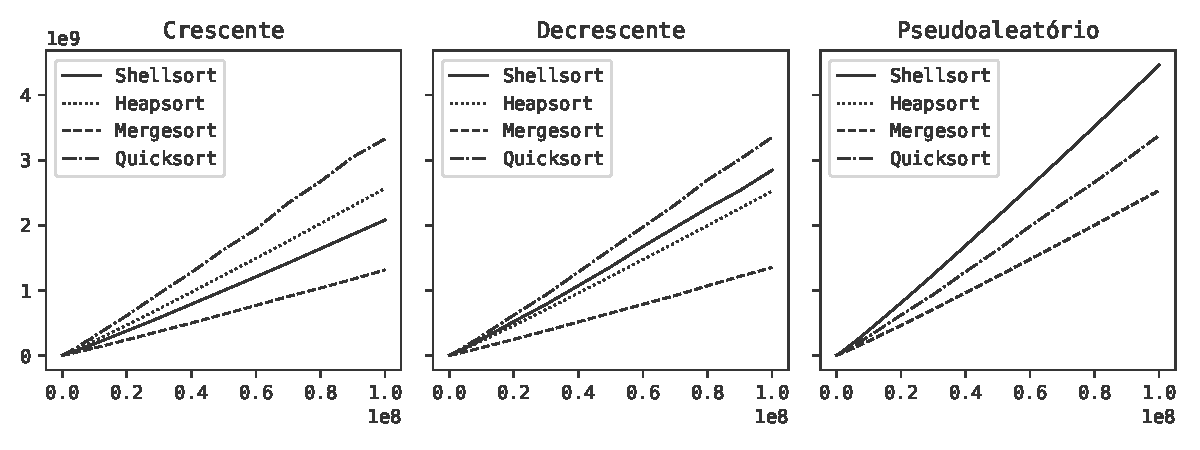
\includegraphics[scale=0.787]{figuras/pdf/superiores.comparacoes.pdf}
\Fonte{Elaborado pelo autor}
\end{figure}

Em contraste com os demais, o Quicksort e o Heapsort demonstraram estabilidade em seu desempenho. Em todos os tipos de vetor, os gráficos de ambos os algoritmos são praticamente idênticos, o que indica que a ordem inicial dos dados não os beneficia nem os prejudica. No entanto, o Heapsort executa um número ligeiramente menor de comparações do que o Quicksort.

Já o Shellsort apresentou um desempenho variável conforme o tipo de vetor. Apesar de se beneficiar quando há presença de ordem nos dados, ele foi, no caso geral, o algoritmo superior que mais executou comparações.

O Mergesort executa o menor número de comparações para todos os três tipos de vetor analisados, destacando-se em vetores já ordenados. Há uma explicação interessante para este fato: o algoritmo Mergesort só executa comparações durante o processo de Merge, e este processo se torna determinístico para vetores ordenados. Esse trecho do algoritmo é mostrado abaixo.

\lstinputlisting[language=C]{codigos/aux/merge_snippet.txt}

\subsection{Movimentações}
O gráfico da Figura \ref{fig:superiores.movimentacoes} a seguir, exibe a relação entre o número de movimentações e o tamanho do vetor para cada tipo de vetor analisado.

\begin{figure}[H]
\Caption{\label{fig:superiores.movimentacoes}Métodos superiores – Tamanho × Movimentações.}
\centering
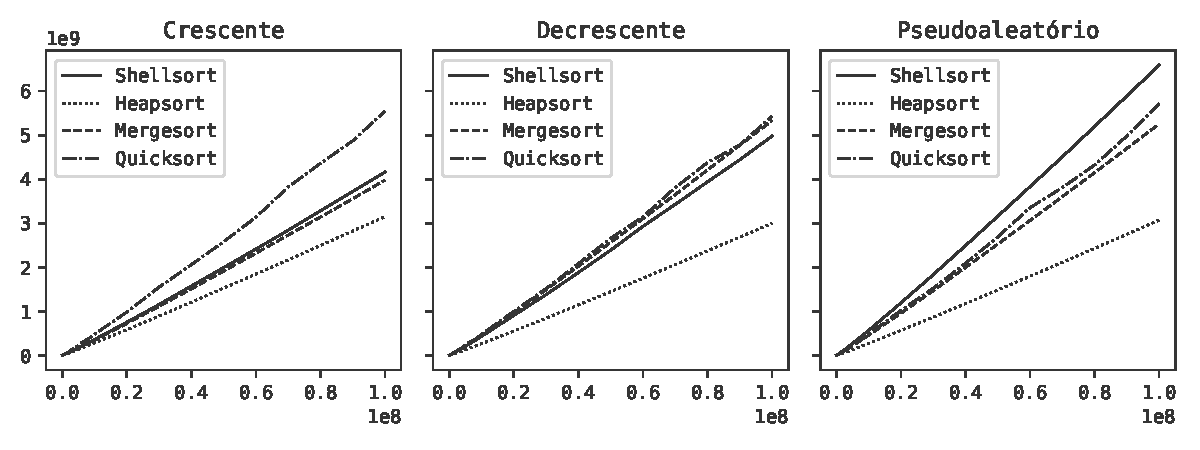
\includegraphics[scale=0.787]{figuras/pdf/superiores.movimentacoes.pdf}
\Fonte{Elaborado pelo autor}
\end{figure}

Com relação à quantidade de movimentações, o algoritmo Heapsort se destacou. Ele manteve o mesmo desempenho em todos os tipos de vetor, mas executou significativamente menos movimentações que os demais algoritmos superiores. O Quicksort também teve desempenho estável para todos os tipos de vetores, sendo ele o que mais executa movimentações para entradas já ordenadas de alguma forma. Já o Mergesort apresentou o mesmo desempenho em vetores decrescentes e no caso geral, mas executou menos movimentações para vetores crescentes, o que ocorre pelo mesmo motivo explicado na subseção anterior. De modo geral, o Shellsort é o que mais realiza a operação de movimentação de elementos do vetor de entrada.

\subsection{Eficiência de cache}\label{subsec:sup-cache}
Conforme introduzido na seção \ref{sec:arquitetura}, o processador tenta realizar a leitura e a escrita primeiramente no cache. Somente quando a informação de interesse não está presente em nenhum nível de cache, é que ele a busca na memória principal. Devido aos tamanhos de vetores utilizados neste trabalho, não é necessário mencionar a memória secundária, uma vez que toda a informação cabe na memória principal. A eficiência de cache de um algoritmo é, portanto, a taxa de sucesso na busca por elementos no cache, visto que esse acesso é muito mais rápido do que na RAM.

\subsubsection{Falhas de leitura}
O gráfico da Figura \ref{fig:superiores-DLmr} mostra a frequência em que o processador falhou ao tentar ler um dado no último nível de cache para cada algoritmo. Observe que, para vetores de tamanhos até $10^7$, e dadas as propriedades do computador utilizado nos testes, praticamente todas as leituras resultavam em sucesso. No entanto, para vetores maiores que isso, as falhas se tornaram visíveis, com o Heapsort sendo o algoritmo que mais apresentou falhas de leitura.

A explicação para a ineficiência do Heapsort reside no princípio da localidade de referência espacial, conforme detalhado na subseção \ref{subsec:localidade-referencia}. Isso ocorre porque, à medida que o algoritmo desce pelos nós do Heap, o índice de cada posição acessada é pelo menos o dobro do índice da posição acessada anteriormente. Essa característica força o carregamento de elementos novos e distantes no cache, os quais se tornam inúteis já na próxima iteração.

\begin{figure}[H]
    \Caption{\label{fig:superiores-DLmr}Métodos superiores – Falhas de leitura no último nível de cache.}
    \centering
    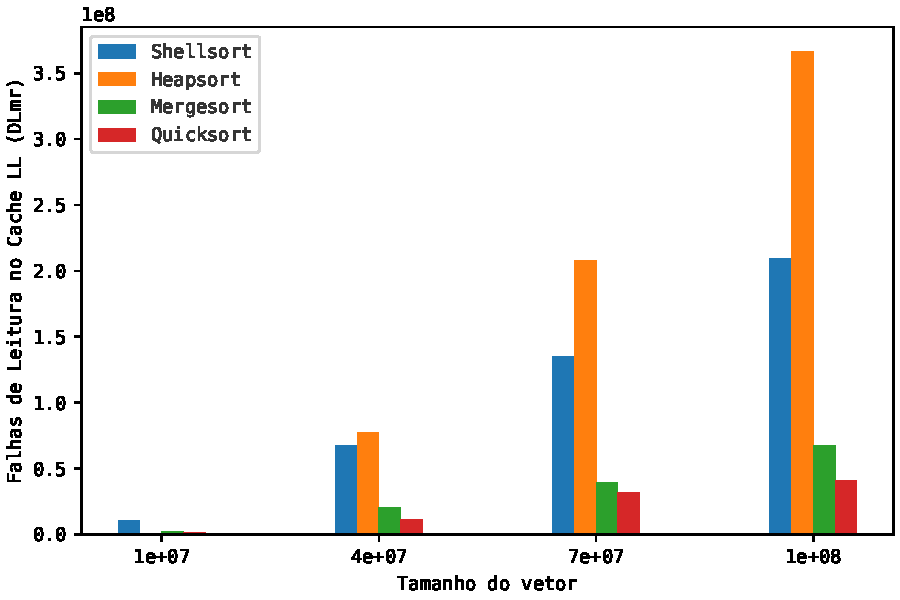
\includegraphics[scale=0.787]{figuras/pdf/superiores_DLmr.pdf}
    \Fonte{Elaborado pelo autor}
\end{figure}

\subsubsection{Falhas de escrita}
O gráfico da Figura \ref{fig:superiores-DLmw} mostra a frequência em que o processador falhou ao tentar escrever um dado no último nível de cache para cada algoritmo. Percebe-se que, mais uma vez, a quantidade de falhas é insignificante para vetores menores que $10^7$. Constata-se também que apenas o Mergesort causa falhas desse tipo. Este fato é explicado pela necessidade deste algoritmo de usar memória auxiliar.

\begin{figure}[H]
\Caption{\label{fig:superiores-DLmw}Métodos superiores – Falhas de escrita no último nível de cache.}
\centering
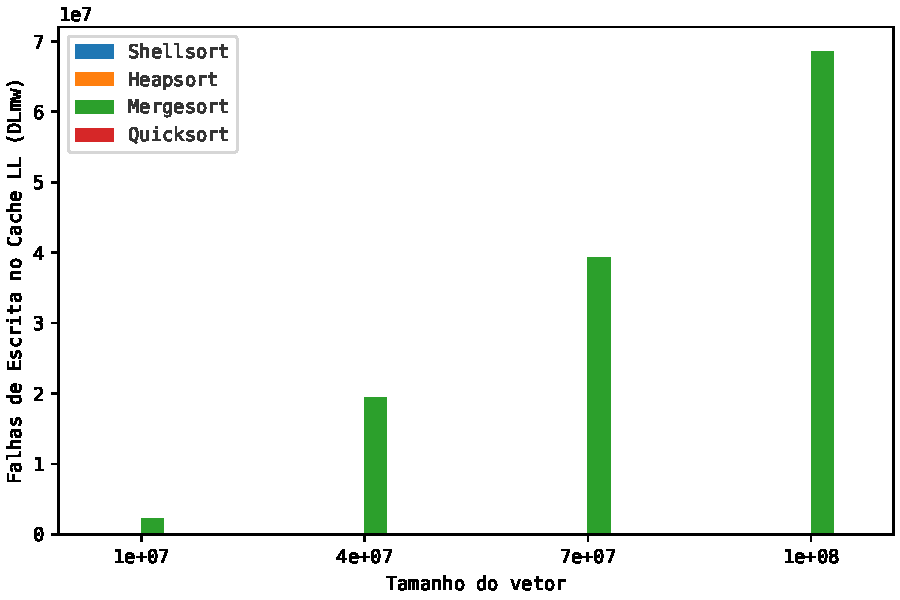
\includegraphics[scale=0.787]{figuras/pdf/superiores_DLmw.pdf}
\Fonte{Elaborado pelo autor}
\end{figure}

\subsection{Síntese dos resultados}
A Table \ref{tab:sup-classicacao} a seguir classifica os algoritmos superiores por tempo, comparações, movimentações e uso do cache, no caso geral.

\begin{table}[H]
    \centering
    \Caption{\label{tab:sup-classicacao}Métodos superiores – Classificação de desempenho por métrica}
    \begin{tabular}{ | c | l | l | l | l | l | }
        \hline
        Ranking & Tempo     & Comp.     & Movi.     & Leitura   & Escrita   \\
        \hline
        1º      & Quicksort & Mergesort & Heapsort  & Quicksort & Shellsort \\
        2º      & Mergesort & Heapsort  & Mergesort & Mergesort & Heapsort  \\
        3º      & Shellsort & Quicksort & Quicksort & Shellsort & Quicksort \\
        4º      & Heapsort  & Shellsort & Shellsort & Heapsort  & Mergesort \\
        \hline
    \end{tabular}
\end{table}

O Quicksort, apesar de não ser o algoritmo que realiza menos comparações ou movimentações, é o mais eficiente em termos de cache. Essa eficiência o estabelece como o melhor algoritmo superior para a principal métrica, o tempo. Já o Shellsort é o que mais executa comparações e movimentações, mas ainda assim acaba sendo mais rápido que o Heapsort, também devido à sua eficiência de cache. Por fim, o Mergesort é quase tão bom quanto o Quicksort, sendo penalizado pelo uso de memória extra.

\section{Quicksort e métodos híbridos}
Os algoritmos de ordenação mais utilizados na prática são híbridos, baseados no Quicksort. Tais algoritmos se beneficiam dos pontos positivos do Quicksort ao mesmo tempo em que tentam diminuir o número de movimentações realizadas e evitar o pior caso.

No capítulo anterior, foram apresentados dois algoritmos desse tipo: o QuicksortI, que utiliza a Inserção para finalizar a ordenação, reduzindo o número de movimentações; e o Introsort, algoritmo utilizado na biblioteca padrão da linguagem de programação C\raisebox{0.4ex}{\text{\tiny{++}}}.

O Introsort também utiliza a Inserção para finalizar a ordenação, mas usa o Heapsort quando a árvore de recursão atinge altura igual a $2\log n$, contornando assim os casos em que o Quicksort tende ao pior cenário. O gráfico da Figura \ref{fig:hibridos} a seguir mostra os resultados de tempo e movimentações do Quicksort em comparação com o QuicksortI e o Introsort. Os resultados com relação ao número de comparações foram equivalentes e, por isso, não serão mostrados.

\begin{figure}[H]
\Caption{\label{fig:hibridos}Métodos híbridos – Tempo e movimentações.}
\centering
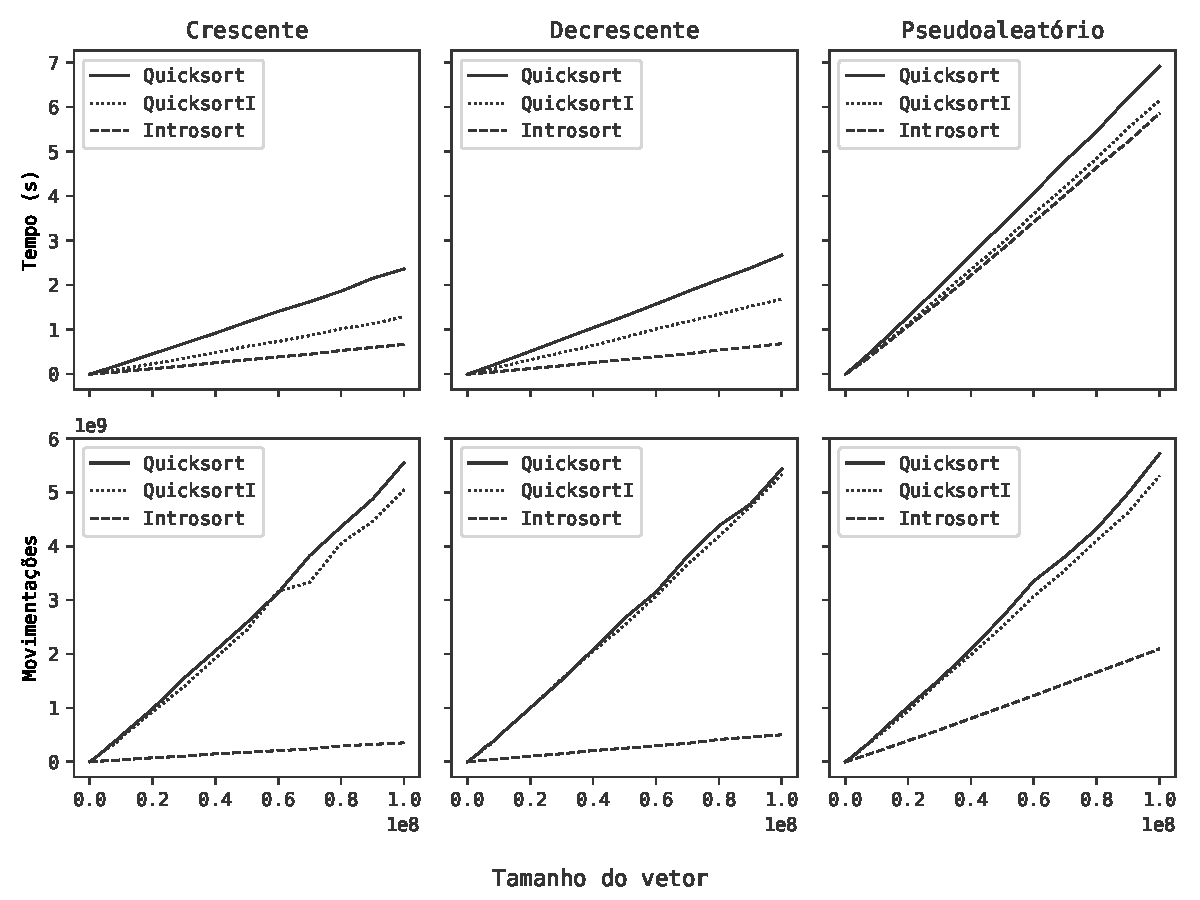
\includegraphics[scale=0.787]{figuras/pdf/hibridos.pdf}
\Fonte{Elaborado pelo autor}
\end{figure}

\section{Métodos lineares}
A subseção \ref{subsec:cota-inferior} mostrou que a cota inferior para algoritmos baseados em comparação é $\Omega(n\log_2n)$. Isso significa que, para um algoritmo ser linear, ele não pode se basear em comparação. Além disso, os algoritmos lineares de ordenação apresentados neste trabalho só são lineares para entradas que obedecem a certas propriedades. Por exemplo, o Countingsort assume que os elementos da entrada podem ser indexados e que a diferença entre o maior e o menor elemento é limitada por uma constante suficientemente pequena para caber na memória. Já o Bucketsort requer que os elementos estejam uniformemente distribuídos em um intervalo. Por fim, o Radixsort assume que o algoritmo auxiliar é estável e linear e que cada elemento da entrada pode ser decomposto em dígitos pertencentes a um conjunto limitado e ordenável. Todos esses pré-requisitos foram levados em consideração nos testes, e todos os vetores foram gerados de modo a manter a característica linear de cada algoritmo.

\begin{figure}[H]
\Caption{\label{fig:lineares}Métodos lineares – Tempo e movimentações.}
\centering
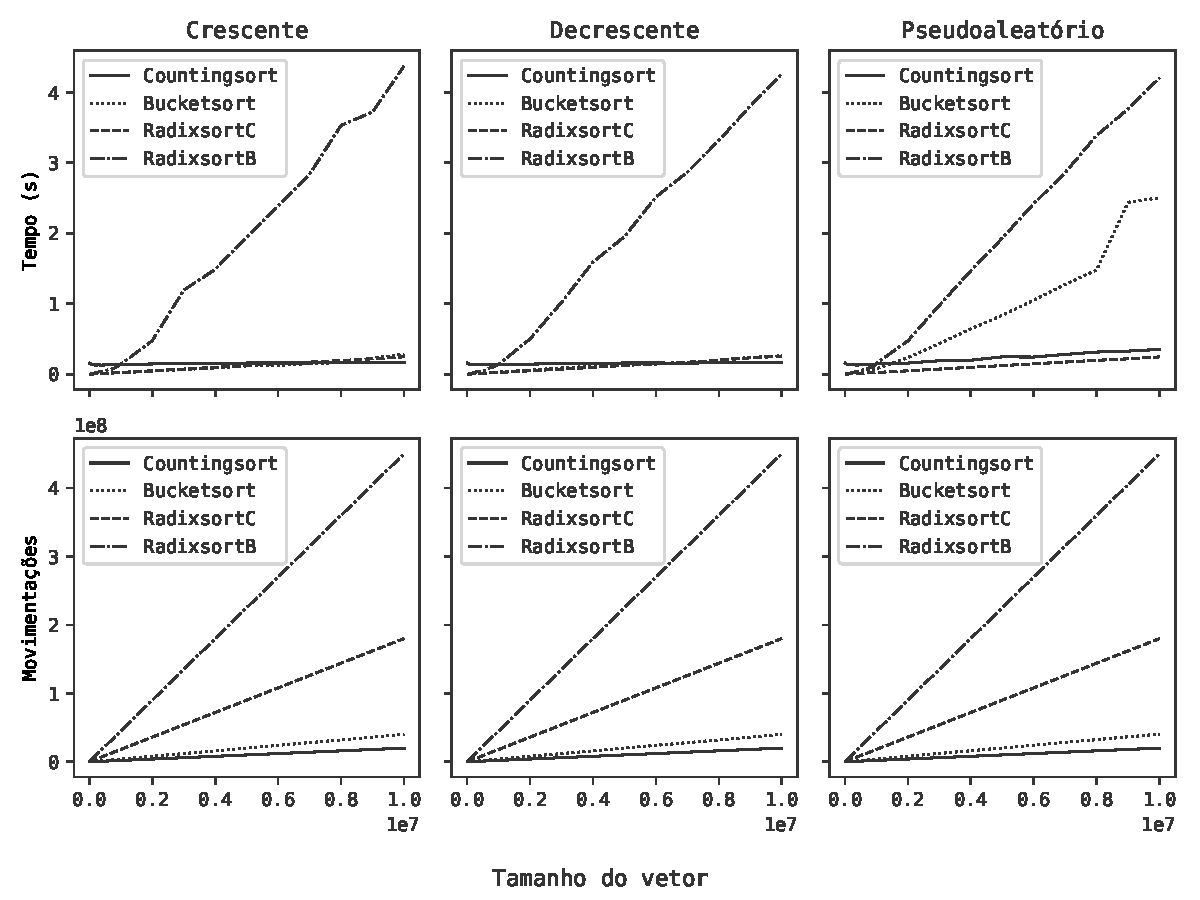
\includegraphics[scale=0.787]{figuras/pdf/lineares.pdf}
\Fonte{Elaborado pelo autor}
\end{figure}

O primeiro ponto a se observar é que cada algoritmo apresenta consistência no número de movimentações. Isso ocorre porque cada um deles, independentemente do tipo de vetor, move os dados para a memória auxiliar e, em seguida, os traz de volta para o vetor de entrada, de modo a garantir a ordenação.

No entanto, ambas as versões do Radixsort — tanto a que usa o Countingsort como sub-rotina quanto a que usa o Bucketsort — executam mais movimentações. Isso se deve ao fato de que elas têm que realizar a movimentação para a memória auxiliar nove vezes, pois essa é a quantidade máxima de dígitos que cada número da entrada pode ter.

Por fim, observamos outros dois comportamentos que o gráfico não explica. O primeiro é que o RadixsortC foi mais rápido que o Countingsort, mesmo executando mais movimentações. Isso ocorre porque o RadixsortC utiliza menos memória que o Countingsort, uma vez que o vetor que armazenaria a frequência de cada elemento da entrada no Countingsort aloca $10^8$ posições, enquanto que no RadixsortC aloca apenas $10$.

O segundo é que o Bucketsort se tornou consideravelmente mais lento para vetores gerados de forma pseudoaleatória. Isso ocorre porque, mesmo que os elementos tendam a ser igualmente prováveis na geração do vetor, não é o que ocorre exatamente na prática. Para vetores crescentes ou decrescentes, devido à forma como os elementos foram escolhidos na geração dos vetores, cada bucket recebeu entre $0$ e $2$ elementos, o que não sobrecarrega a versão do Insercao utilizada. Já para vetores gerados de forma pseudoaleatória, os buckets tiveram entre $0$ e $9$ elementos, como mostra a Figura \ref{fig:frequencia-buckets}. Esse desequilíbrio fez com que o Insercao precisasse executar mais operações na lista ligada utilizada, o que tornou o algoritmo mais lento nesses casos.

\begin{figure}[H]
\Caption{\label{fig:frequencia-buckets}Bucketsort – Frequência de tamanho de bucket ($10^7$ elementos)}
\centering
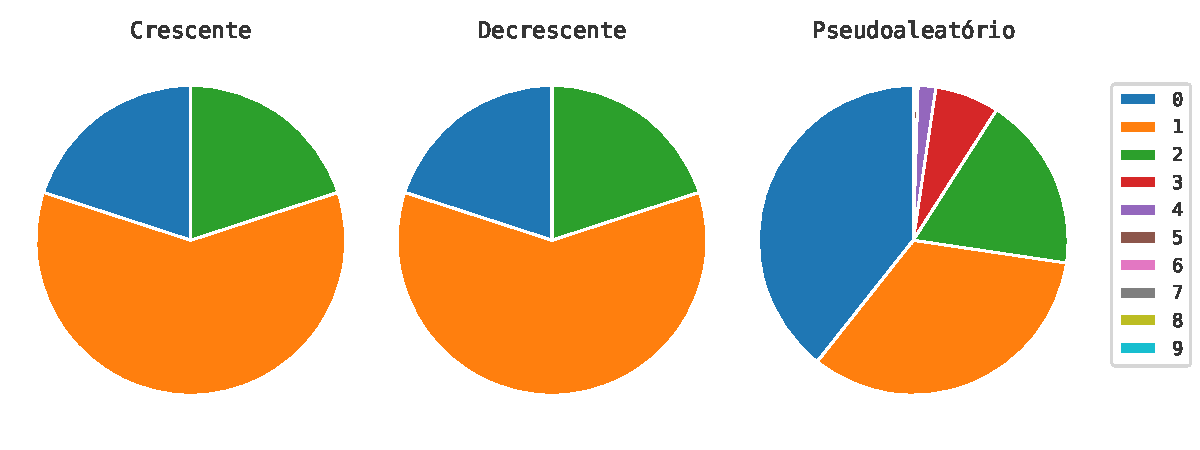
\includegraphics[scale=0.787]{figuras/pdf/frequencia_buckets.pdf}
\Fonte{Elaborado pelo autor}
\end{figure}
